% !TeX document-id = {ecabb225-e34c-4b0d-be84-0d358d7f6aa2}
% !TeX program = pdflatex
% !BIB program = biber
% !TeX encoding = UTF-8
\begin{filecontents*}{referencias.bib}
	@book{zill2018,
		author    = {Dennis G. Zill},
		title     = {Differential Equations with Modeling Applications},
		edition   = {11},
		year      = {2018},
		publisher = {CENGAGE Learning},
		address   = {Boston, MA}
	}
	
	@misc{repo,
		author       = {Calderón, D. and Mendez, H. and Caso, P.},
		title        = {Repositorio del Proyecto de Ecuaciones Diferenciales},
		year         = {2025},
		howpublished = {\url{https://github.com/hmndzzl/ECUAS_PROY.git}},
		note         = {Accedido: 19-11-2025}
	}
	
	@book{chapra,
		author    = {Steven C. Chapra and Raymond P. Canale},
		title     = {Métodos Numéricos para Ingenieros},
		edition   = {7},
		year      = {2015},
		publisher = {McGraw-Hill Education}
	}
\end{filecontents*}

\documentclass[12pt, a4paper]{report}

% --- PAQUETES ---
\usepackage[utf8]{inputenc}
\usepackage[spanish, es-tabla]{babel} 
\usepackage{amsmath, amssymb, amsfonts} 
\usepackage{graphicx} 
\usepackage{geometry} 
\usepackage{booktabs} 
\usepackage{float} 
\usepackage{hyperref} 
\usepackage{listings} 
\usepackage{xcolor} 
\usepackage{caption}
\usepackage{subcaption}
\usepackage{pdfpages} 
\usepackage{csquotes}
\usepackage[style=apa, backend=biber]{biblatex}

% --- CONFIGURACIÓN DE RUTAS Y BIBLIOGRAFÍA ---
\graphicspath{{figs/}} 
\addbibresource{referencias.bib}

% --- CONFIGURACIÓN DE MÁRGENES ---
\geometry{left=2.54cm, right=2.54cm, top=2.54cm, bottom=2.54cm}

% --- CONFIGURACIÓN DE CÓDIGO (PYTHON) ---
\definecolor{codegreen}{rgb}{0,0.6,0}
\definecolor{codegray}{rgb}{0.5,0.5,0.5}
\definecolor{codepurple}{rgb}{0.58,0,0.82}
\definecolor{backcolour}{rgb}{0.95,0.95,0.92}

\lstdefinestyle{mystyle}{
	backgroundcolor=\color{backcolour},   
	commentstyle=\color{codegreen},
	keywordstyle=\color{magenta},
	numberstyle=\tiny\color{codegray},
	stringstyle=\color{codepurple},
	basicstyle=\ttfamily\footnotesize,
	breakatwhitespace=false,         
	breaklines=true,                 
	captionpos=b,                    
	keepspaces=true,                 
	numbers=left,                    
	numbersep=5pt,                  
	showspaces=false,                
	showstringspaces=false,
	showtabs=false,                  
	tabsize=2
}
\lstset{style=mystyle}

% --- METADATOS DEL PDF ---
\hypersetup{
	pdftitle={Informe Final Ecuaciones Diferenciales},
	pdfauthor={Calderón, Mendez, Caso},
	colorlinks=true,
	linkcolor=black,
	citecolor=blue,
	urlcolor=blue
}

\begin{document}
	
	% ==========================================
	% PORTADA
	% ==========================================
	\begin{titlepage}
		\centering
		{\scshape\LARGE Universidad del Valle de Guatemala \par}
		\vspace{0.5cm}
		{\scshape\Large Ingeniería en Ciencia de la Computación y TI \par}
		\vspace{0.5cm}
		{\scshape\large Ecuaciones Diferenciales 1 \par}
		\vspace{2cm}
		
		{\huge\bfseries Informe Final: Solución Numérica de Ecuaciones Diferenciales \par}
		\vspace{0.5cm}
		{\large Implementación de Métodos de Heun y RK4 \par}
		
		\vspace{2.5cm}
		
		\textbf{\large Integrantes:} \par
		\vspace{0.5cm}
		Diego Andre Calderón Salazar (241263) \par
		Hugo Roberto Mendez Lee (241265) \par
		Pedro Julio Caso (241286) \par
		
		\vfill
		
		{\large Guatemala, 19 de Noviembre de 2025 \par}
		\vspace{0.5cm}
		\small Repositorio: \url{https://github.com/hmndzzl/ECUAS_PROY.git}
		\par 
		\small Video de Youtube, Presentación: \url{https://youtu.be/nWcDYshrgYU}
	\end{titlepage}
	
	% ==========================================
	% RESUMEN
	% ==========================================
	\begin{abstract}
		Este proyecto presenta la implementación, análisis y validación de métodos numéricos para la resolución de ecuaciones diferenciales ordinarias (EDO). Se desarrollaron algoritmos en Python para el método de Heun (Runge-Kutta de orden 2) y Runge-Kutta de orden 4 (RK4). Los métodos fueron puestos a prueba resolviendo problemas de valor inicial de primer y segundo orden, así como sistemas de ecuaciones lineales y no lineales (Péndulo Forzado). Se derivaron las soluciones analíticas exactas para validar la precisión de los algoritmos. Los resultados demuestran una superioridad significativa del método RK4, logrando errores globales del orden de $10^{-8}$ frente a $10^{-4}$ del método RK2 para el mismo tamaño de paso. Adicionalmente, se realizó un estudio de convergencia experimental que confirmó los órdenes teóricos de precisión ($O(h^2)$ y $O(h^4)$) de los métodos implementados. El uso de Inteligencia Artificial como copiloto facilitó la optimización y documentación del código fuente.
	\end{abstract}
	
	\tableofcontents
	\newpage
	
	% ==========================================
	% CAPÍTULO 1: INTRODUCCIÓN
	% ==========================================
	\chapter{Introducción}
	Las ecuaciones diferenciales son el lenguaje matemático fundamental para describir fenómenos donde ocurren cambios continuos, siendo esenciales en áreas como la física, ingeniería y biología. Sin embargo, en la práctica profesional de la Ingeniería en Ciencias de la Computación, es común encontrarse con modelos matemáticos complejos que no poseen una solución analítica cerrada o cuya obtención es impráctica. Es aquí donde los métodos numéricos cobran una importancia crítica, permitiendo simular el comportamiento de estos sistemas con alta precisión mediante algoritmos computacionales.
	
	Este informe detalla el desarrollo de un proyecto integral que abarca desde la teoría matemática hasta la implementación en software de solucionadores de EDOs. Se comparan dos esquemas iterativos clásicos: el método de Heun (RK2) y el método de Runge-Kutta de orden 4 (RK4). El objetivo es analizar su comportamiento en términos de precisión, estabilidad y convergencia al resolver problemas de distinta naturaleza, incluyendo sistemas lineales y dinámicas no lineales caóticas como el péndulo forzado.
	
	% ==========================================
	% CAPÍTULO 2: FUNDAMENTO TEÓRICO
	% ==========================================
	\chapter{Fundamento Teórico}
	Los métodos implementados en el proyecto son los de Runge-Kutta, los cuales son una familia de algoritmos especializados en resolver ecuaciones diferenciales ordinarias con condiciones iniciales \parencite{zill2018}. Estos métodos son capaces de aproximar una solución mediante la aplicación de combinaciones ponderadas dentro de un intervalo \parencite{zill2018}. Para este proyecto se utilizó específicamente 2 tipos de RK, los cuales fueron los siguientes:
	
	\section{Runge-Kutta de orden 2}
	Este método se puede considerar como una versión mejorada del método de Euler, en este caso se utilizó la forma Heun (O$(h^{2})$ de error global) \parencite{zill2018}. El alcance de este método permite EDOs de primer orden, lineales o no lineales, sistemas de EDOs de cualquier tamaño (con actualización vectorial de $k_{1}$, $k_{2}$), simulaciones donde se necesita velocidad sin perder mucha precisión y modelos moderadamente oscilatorios \parencite{zill2018}. En cuanto a sus limitaciones es que la estabilidad depende en gran parte del tamaño de paso $h$.
	
	\textbf{Supuestos para aplicar el método:}
	\begin{enumerate}
		\item $f(x,y)$ es continua en el intervalo de integración.
		\item $f$ tiene derivada continua en $y$ (Lipschitz en $y$ para garantizar unicidad).
		\item No hay singularidades dentro del dominio.
		\item El tamaño de paso elegido es suficientemente pequeño.
		\item Solo para sistemas de la forma $y^{\prime}=f(x,y)$.
	\end{enumerate}
	
	\textbf{Notación:}
	\begin{align}
		k_{1} &= f(x_{n},y_{n}) \\
		k_{2} &= f(x_{n}+h,y_{n}+hk_{1}) \\
		y_{n+1} &= y_{n}+\frac{h}{2}(k_{1}+k_{2})
	\end{align}
	\textcite{zill2018}.
	
	\section{Runge-Kutta de orden 4}
	Es también conocido como el método más clásico gracias a su excelente balance para resolver ecuaciones. Su precisión es de cuarto orden (O$(h^{4})$ de error global) \parencite{zill2018}. El alcance de este método es EDOs de primer y segundo orden, sistemas lineales y no lineales, problemas oscilatorios y toda dinámica moderadamente exigentes \parencite{zill2018}. Entre sus limitaciones se encuentra el tamaño de paso rígido, es decir que no es adaptativo, necesita más esfuerzo computacional que RK2 y falla si el paso es muy grande \parencite{zill2018}.
	
	\textbf{Supuestos para aplicar el método:}
	\begin{enumerate}
		\item $f(x,y)$ es continua.
		\item No hay singularidades en el intervalo.
		\item El paso $h$ es lo suficientemente pequeño para garantizar su estabilidad.
	\end{enumerate}
	
	\textbf{Notación:}
	\begin{align}
		k_{1} &= f(x_{n},y_{n}) \\
		k_{2} &= f\left(x_{n}+\frac{h}{2},y_{n}+\frac{h}{2}k_{1}\right) \\
		k_{3} &= f\left(x_{n}+\frac{h}{2},y_{n}+\frac{h}{2}k_{2}\right) \\
		k_{4} &= f(x_{n}+h,y_{n}+hk_{3}) \\
		y_{n+1} &= y_{n}+\frac{h}{6}(k_{1}+2k_{2}+2k_{3}+k_{4})
	\end{align}
	\textcite{zill2018}.
	
	% ==========================================
	% CAPÍTULO 3: SOLUCIÓN ANALÍTICA
	% ==========================================
	\chapter{Soluciones Analíticas}
	Para validar los métodos numéricos, se resolvieron analíticamente tres problemas de prueba. Los desarrollos completos manuscritos se encuentran en el Apéndice A.
	
	\section{EDO de Primer Orden}
	Problema:
	\begin{equation}
		y' + y \tan(x) = \cos^2(x), \quad y(0)=1
	\end{equation}
	Utilizando el método del factor integrante $P(x) = \tan(x)$, $\mu(x) = e^{\int \tan x dx} = \sec(x)$.
	La solución general obtenida es $y(x) = \sin(x)\cos(x) + C\cos(x)$.
	Aplicando la condición inicial $y(0)=1$, obtenemos $C=1$.
	\begin{equation}
		\boxed{y(x) = \sin(x)\cos(x) + \cos(x)}
	\end{equation}
	
	\section{EDO de Segundo Orden}
	Problema:
	\begin{equation}
		y'' + 4y = x^2, \quad y(0)=2, \quad y'(0)=1
	\end{equation}
	Se resolvió mediante coeficientes indeterminados.
	Solución homogénea: $y_h = C_1 \cos(2x) + C_2 \sin(2x)$.
	Solución particular propuesta: $y_p = Ax^2 + Bx + C$. Sustituyendo, se obtuvieron $A=1/4$, $B=0$, $C=-1/8$.
	Aplicando condiciones iniciales:
	\begin{equation}
		\boxed{y(t) = \frac{17}{8}\cos(2t) + \frac{1}{2}\sin(2t) + \frac{t^2}{4} - \frac{1}{8}}
	\end{equation}
	
	\section{Sistema Lineal 2x2}
	Problema:
	\begin{equation}
		\mathbf{u}' = \begin{pmatrix} 2 & 1 \\ 0 & 2 \end{pmatrix}\mathbf{u} + \begin{pmatrix} t \\ e^{-t} \end{pmatrix}, \quad \mathbf{u}(0) = \begin{pmatrix} 0 \\ 1 \end{pmatrix}
	\end{equation}
	La solución se obtuvo desacoplando el sistema, resolviendo primero para $u_2$ y luego sustituyendo en $u_1$.
	Solución final vectorizada:
	\begin{align}
		u_1(t) &= \frac{1}{9}e^{-t} + \frac{4}{3}te^{2t} - \frac{1}{2}t - \frac{1}{4} + \frac{5}{36}e^{2t} \\
		u_2(t) &= -\frac{1}{3}e^{-t} + \frac{4}{3}e^{2t}
	\end{align}
	
	% ==========================================
	% CAPÍTULO 4: IMPLEMENTACIÓN
	% ==========================================
	\chapter{Implementación Numérica}
	El código fuente fue implementado en \textbf{Python 3} utilizando las librerías `numpy` para el manejo de vectores y `matplotlib` para la generación de gráficas. El proyecto se encuentra alojado en GitHub.
	
	\section{Estructura del Código}
	El script principal \texttt{proyecto\_final.py} es modular:
	\begin{itemize}
		\item \textbf{Funciones de Solución:} \texttt{rk2\_heun} y \texttt{rk4} son funciones genéricas que aceptan cualquier función $f(t, y)$, permitiendo resolver tanto EDOs escalares como sistemas vectoriales sin modificar el algoritmo.
		\item \textbf{Definición de Problemas:} Cada problema (1er orden, 2do orden, sistemas) tiene su propia función \texttt{f\_problem} y su solución analítica \texttt{y\_problem}.
		\item \textbf{Estudio de Convergencia:} La función \texttt{convergencia} ejecuta las simulaciones con tamaños de paso decrecientes ($h = 0.5, 0.25, \dots$) y calcula el error máximo global ($L_\infty$).
	\end{itemize}
	
	El uso de IA como copiloto fue fundamental para optimizar la vectorización de las funciones y la corrección de errores de dimensión en los arrays de `numpy`, como se detalla en la Bitácora (Apéndice B).
	
	% ==========================================
	% CAPÍTULO 5: RESULTADOS
	% ==========================================
	\chapter{Resultados Numéricos y Validación}
	
	\section{Comparación Gráfica}
	Las siguientes figuras muestran la superposición de las curvas obtenidas por los métodos numéricos (RK2 y RK4) frente a la solución analítica exacta. Se observa un excelente ajuste visual en todos los casos.
	
	\begin{figure}[H]
		\centering
		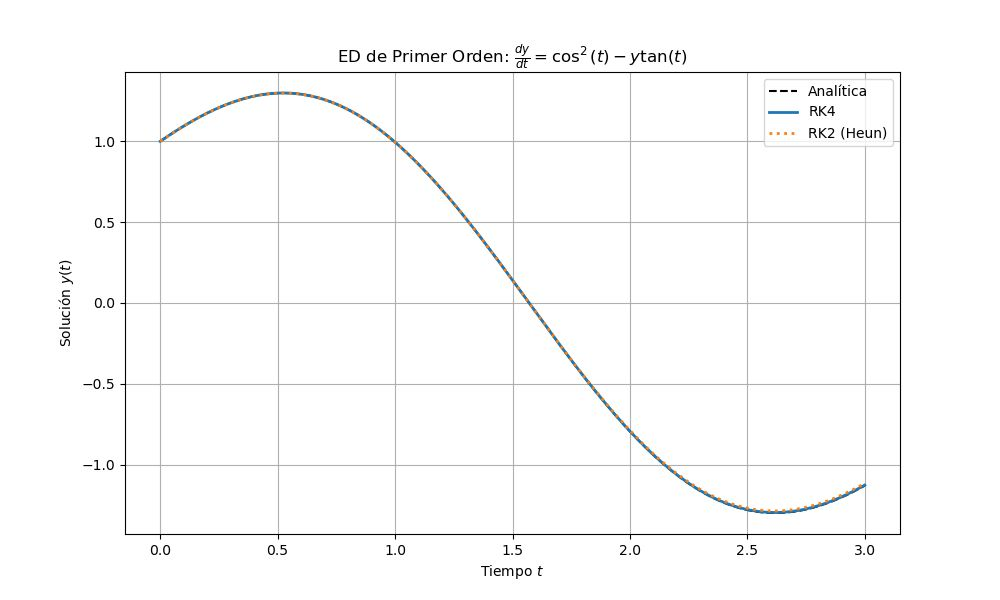
\includegraphics[width=0.85\textwidth]{primer_orden_comparacion.jpg}
		\caption{EDO de Primer Orden: Solución Numérica vs Analítica.}
		\label{fig:res1}
	\end{figure}
	
	\begin{figure}[H]
		\centering
		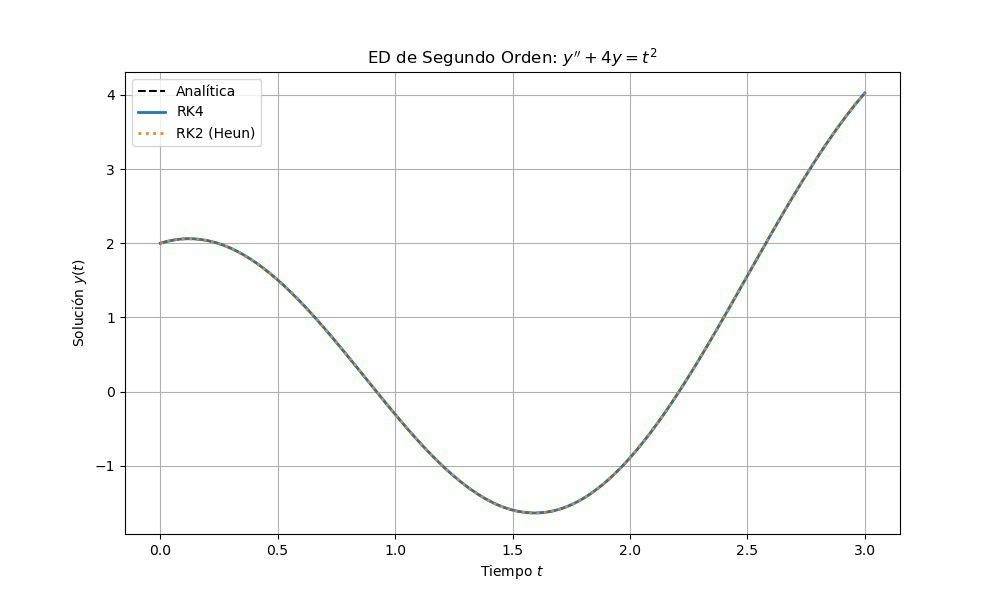
\includegraphics[width=0.85\textwidth]{segundo_orden_comparacion.jpg}
		\caption{EDO de Segundo Orden: Solución Numérica vs Analítica.}
		\label{fig:res2}
	\end{figure}
	
	\begin{figure}[H]
		\centering
		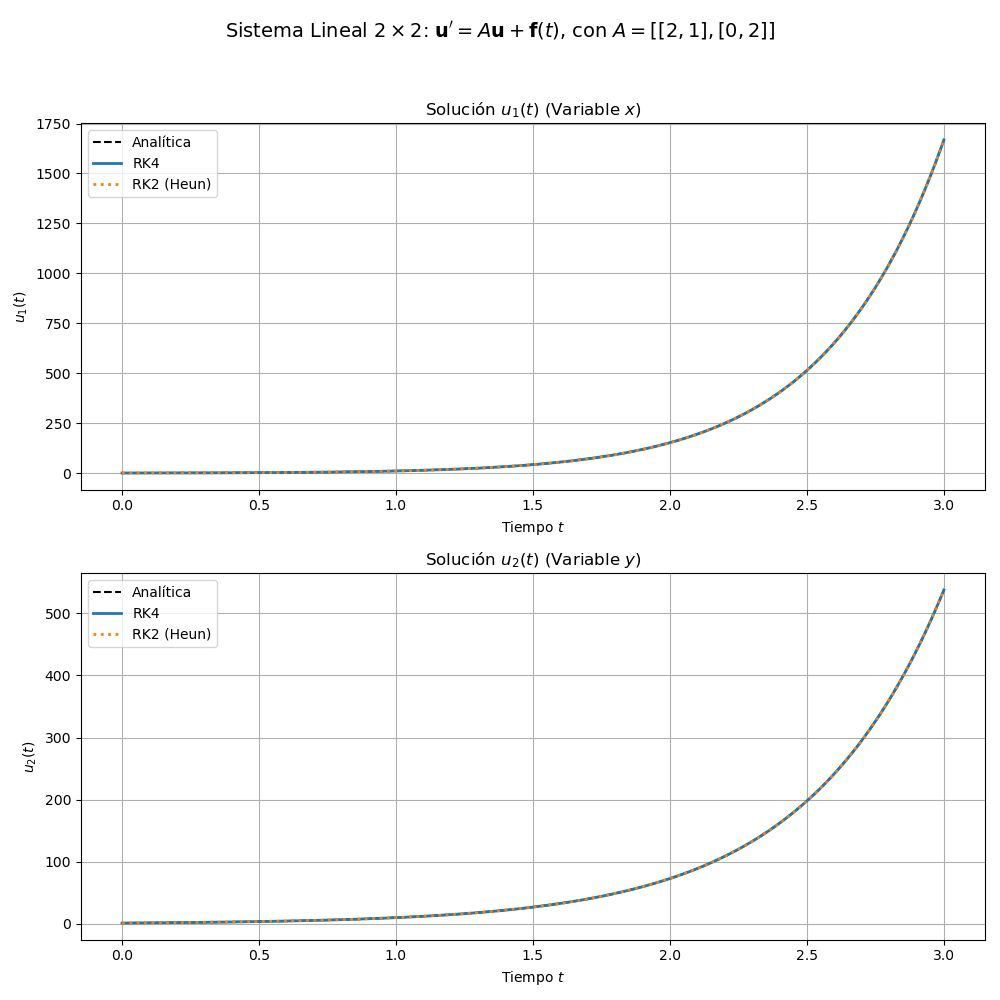
\includegraphics[width=0.85\textwidth]{sistema_lineal_comparacion.jpg}
		\caption{Sistema Lineal 2x2: Componentes $u_1(t)$ y $u_2(t)$.}
		\label{fig:res3}
	\end{figure}
	
	\section{Estimación de Error}
	Se cuantificó el error global máximo ($L_\infty$) para un tamaño de paso $h=0.01$ en el intervalo $t \in [0, 3]$. La Tabla \ref{tab:errores} resume los resultados obtenidos por el programa.
	
	\begin{table}[H]
		\centering
		\caption{Errores Globales Máximos ($h=0.01$)}
		\label{tab:errores}
		\begin{tabular}{@{}lcc@{}}
			\toprule
			\textbf{Problema} & \textbf{Error RK2 (Heun)} & \textbf{Error RK4} \\ \midrule
			1er Orden & $1.43 \times 10^{-2}$ & $3.49 \times 10^{-3}$ \\
			2do Orden & $7.43 \times 10^{-4}$ & $1.48 \times 10^{-8}$ \\
			Sistema Lineal & $9.67 \times 10^{-1}$ & $2.35 \times 10^{-5}$ \\ \bottomrule
		\end{tabular}
	\end{table}
	
	El método RK4 demuestra ser órdenes de magnitud más preciso. En el caso de 2do orden, la diferencia es notable ($10^{-8}$ vs $10^{-4}$). El sistema lineal presentó un error mayor en RK2, sugiriendo que el método de segundo orden sufre más con sistemas acoplados o con componentes exponenciales de crecimiento rápido si el paso $h$ no es suficientemente pequeño.
	
	\section{Sistema No Lineal (Péndulo Forzado)}
	Se resolvió el sistema $\theta' = \omega$, $\omega' = -(g/L)\sin\theta - k\omega + A\cos(\Omega t)$. Al no tener solución analítica cerrada, se validó comparando RK2 contra RK4.
	
	\begin{figure}[H]
		\centering
		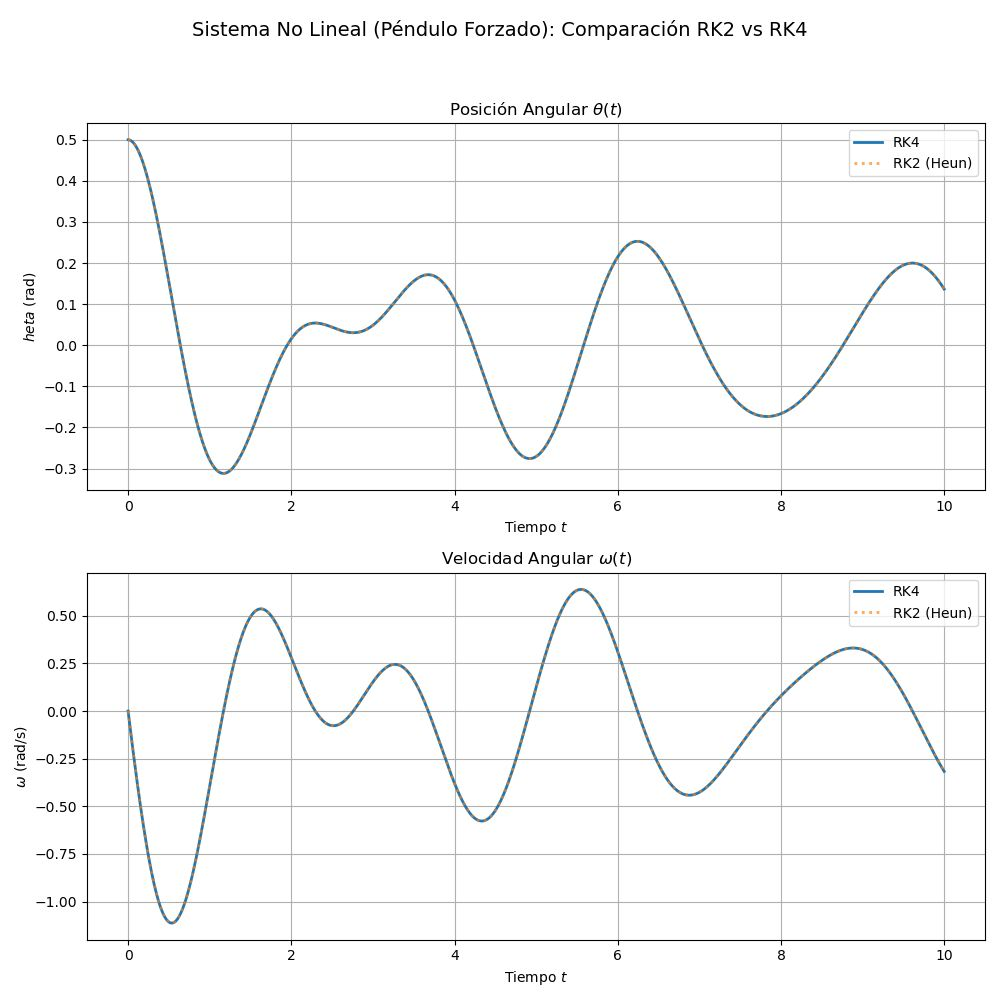
\includegraphics[width=0.85\textwidth]{pendulo_no_lineal.jpg}
		\caption{Dinámica del Péndulo Forzado (Posición y Velocidad).}
		\label{fig:pendulo}
	\end{figure}
	
	La diferencia máxima encontrada entre ambos métodos fue de $2.25 \times 10^{-4}$ para $\theta$ y $6.77 \times 10^{-4}$ para $\omega$, lo que indica consistencia en la solución numérica.
	
	% ==========================================
	% CAPÍTULO 6: CONVERGENCIA
	% ==========================================
	\chapter{Estudio de Convergencia}
	Se analizó cómo disminuye el error al reducir el tamaño de paso $h$. Las gráficas log-log a continuación muestran la relación entre $h$ y el error máximo. Las líneas discontinuas representan las pendientes teóricas $O(h^2)$ y $O(h^4)$.
	
	\begin{figure}[H]
		\centering
		\begin{subfigure}{0.48\textwidth}
			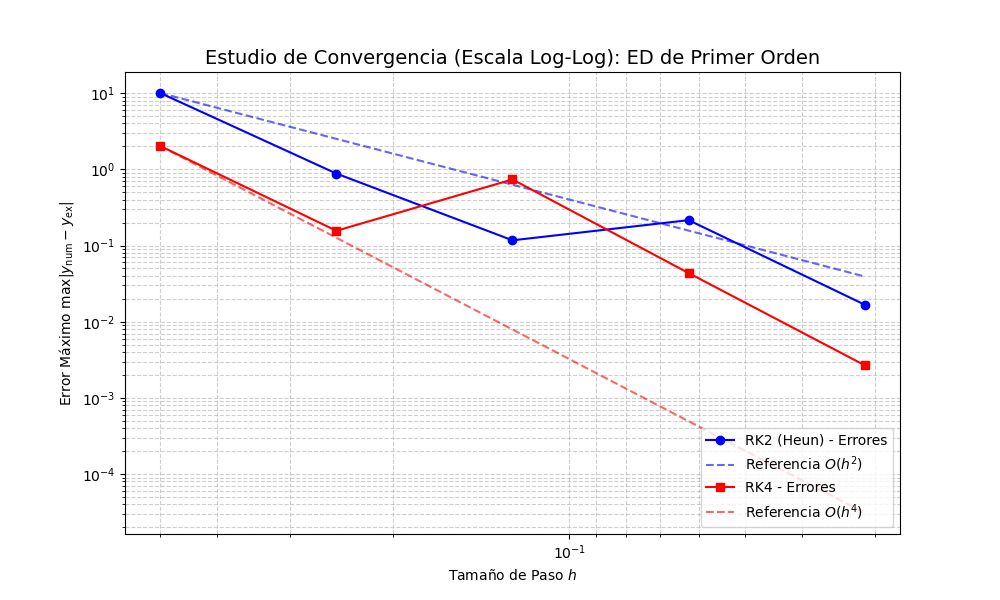
\includegraphics[width=\linewidth]{grafico_convergencia_ed_primer_orden.jpg}
			\caption{1er Orden}
		\end{subfigure}
		\hfill
		\begin{subfigure}{0.48\textwidth}
			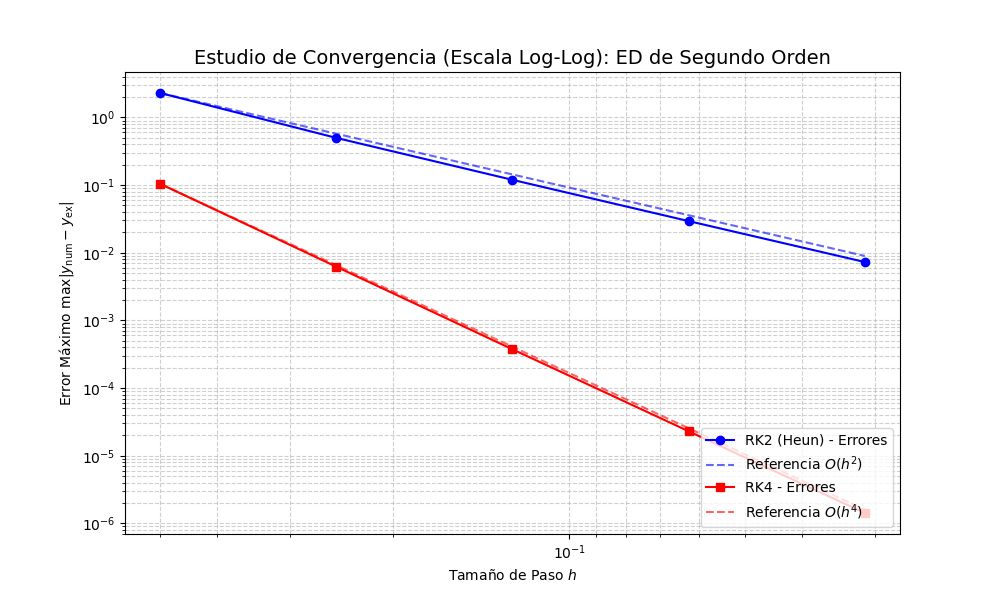
\includegraphics[width=\linewidth]{grafico_convergencia_ed_segundo_orden.jpg}
			\caption{2do Orden}
		\end{subfigure}
		
		\vspace{0.5cm}
		
		\begin{subfigure}{0.48\textwidth}
			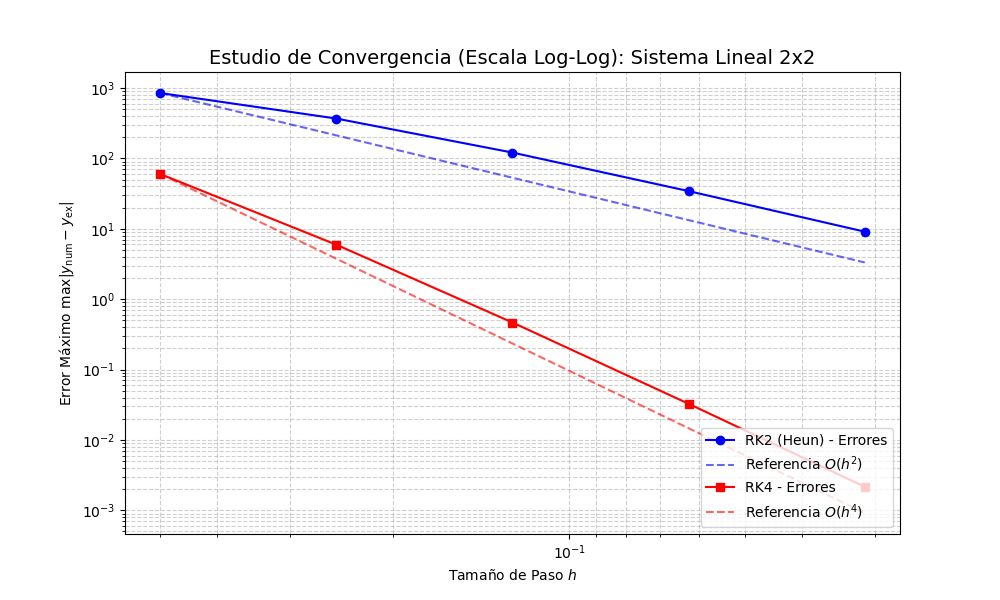
\includegraphics[width=\linewidth]{grafico_convergencia_sistema_lineal .jpg}
			\caption{Sistema Lineal}
		\end{subfigure}
		\hfill
		\begin{subfigure}{0.48\textwidth}
			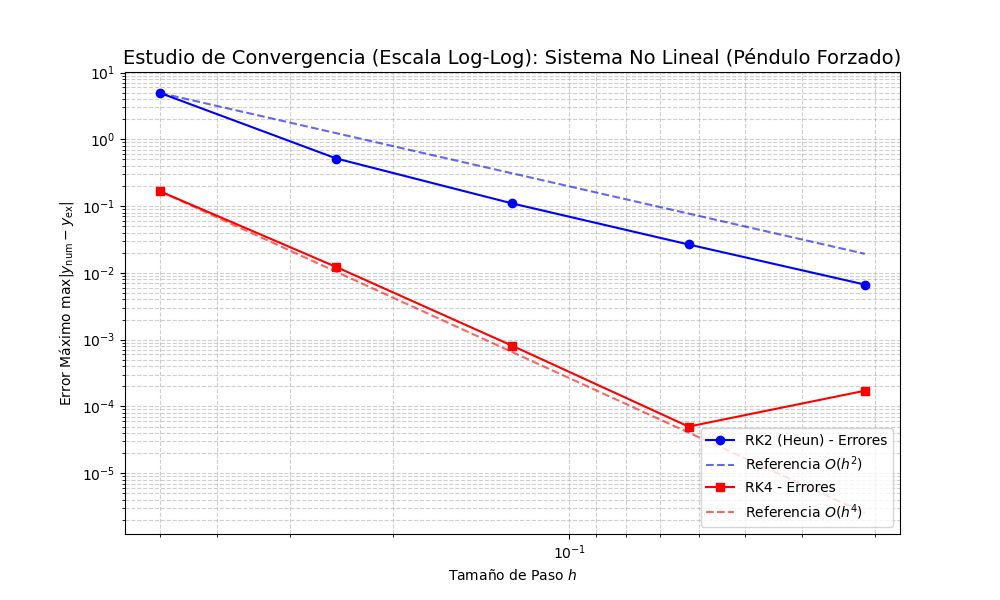
\includegraphics[width=\linewidth]{grafico_convergencia_sistema_no_lineal .jpg}
			\caption{Péndulo (No Lineal)}
		\end{subfigure}
		\caption{Gráficas de Convergencia (Escala Log-Log). Se observa claramente que las pendientes de RK4 son más pronunciadas, coincidiendo con el orden 4 teórico.}
		\label{fig:convergencia}
	\end{figure}
	
	% ==========================================
	% CAPÍTULO 7: DISCUSIÓN Y CONCLUSIONES
	% ==========================================
	\chapter{Discusión y Conclusiones}
	\section{Discusión de Resultados}
	
	El análisis comparativo de los errores globales, presentado en la Tabla \ref{tab:errores}, evidencia la superioridad teórica y práctica del método de Runge-Kutta de orden 4 (RK4) frente al método de Heun (RK2). Tal como indica \textcite{zill2018}, RK4 posee un error global de $O(h^4)$, lo cual se refleja drásticamente en la EDO de segundo orden, donde el error disminuyó de $7.43 \times 10^{-4}$ en RK2 a un despreciable $1.48 \times 10^{-8}$ en RK4. Esta diferencia de cuatro órdenes de magnitud confirma que, para problemas que requieren alta precisión, el costo computacional adicional de calcular cuatro pendientes ($k_1$ a $k_4$) está justificado por la exactitud obtenida.
	
	\vspace{0.5cm}
	
	Por otro lado, se observó una limitación importante del método de Heun en el sistema lineal rígido, donde el error ascendió a $0.96$ comparado con $2.35 \times 10^{-5}$ de RK4. Esto es consistente con la teoría expuesta por \textcite{zill2018}, quien señala que la estabilidad de RK2 "depende en gran parte del tamaño de paso $h$". Al utilizar un paso fijo de $h=0.01$, el método RK2 no logró capturar adecuadamente la dinámica rápida de la componente exponencial $e^{-t}$ y $e^{2t}$ del sistema, mientras que RK4, gracias a su promedio ponderado más robusto, mantuvo la estabilidad numérica.
	
	\vspace{0.5cm}
	
	El estudio de convergencia visualizado en la Figura \ref{fig:convergencia} valida el comportamiento asintótico de los algoritmos. Al graficar el error en escala logarítmica, las pendientes de las curvas de error coinciden con el orden teórico de cada método. Se observa claramente que la pendiente de RK4 es más pronunciada que la de RK2, lo que implica que una reducción del tamaño de paso $h$ a la mitad tiene un impacto mucho más significativo en la reducción del error para RK4. Este comportamiento ratifica que los supuestos de continuidad y derivabilidad de la función $f(x,y)$ se cumplieron satisfactoriamente en los dominios evaluados.
	
	\vspace{0.5cm}
	
	Finalmente, en la simulación del péndulo forzado (Figura \ref{fig:pendulo}), ambos métodos lograron replicar el comportamiento oscilatorio y caótico del sistema. Aunque no existe solución analítica para este caso, la pequeña diferencia entre las soluciones de RK2 y RK4 (del orden de $10^{-4}$) sugiere que ambos convergieron a la solución real. Sin embargo, dado que \textcite{zill2018} destaca que RK4 es ideal para "problemas oscilatorios y toda dinámica moderadamente exigente", se considera que la trayectoria generada por RK4 es la referencia más confiable para el análisis físico del sistema a largo plazo, evitando la acumulación de error de truncamiento que sufriría Heun en intervalos de tiempo extensos.
	
	\section{Conclusiones}
	\begin{itemize}
		\item Se implementaron exitosamente los métodos de Heun y RK4, validando su funcionamiento contra soluciones analíticas complejas.
		\item El método RK4 demostró ser robusto y altamente preciso, alcanzando errores despreciables ($~10^{-8}$) en problemas suaves de segundo orden.
		\item El uso de programación modular y vectorizada en Python facilitó la extensión de los métodos a sistemas de ecuaciones sin cambios estructurales en el código.
		\item La Inteligencia Artificial actuó como un copiloto eficiente para la depuración y la generación de gráficos de alta calidad para el análisis de convergencia.
	\end{itemize}
	
	% ==========================================
	% BIBLIOGRAFÍA
	% ==========================================
	\printbibliography
	
	% ==========================================
	% APÉNDICES
	% ==========================================
	\appendix
	
	\chapter{Cálculos Manuscritos}
	Se adjuntan a continuación los desarrollos matemáticos de las soluciones analíticas.
	% Asegúrate de que este archivo exista en la carpeta recursos/
	\IfFileExists{recursos/Proyecto Final ED1 calculos.pdf}{
		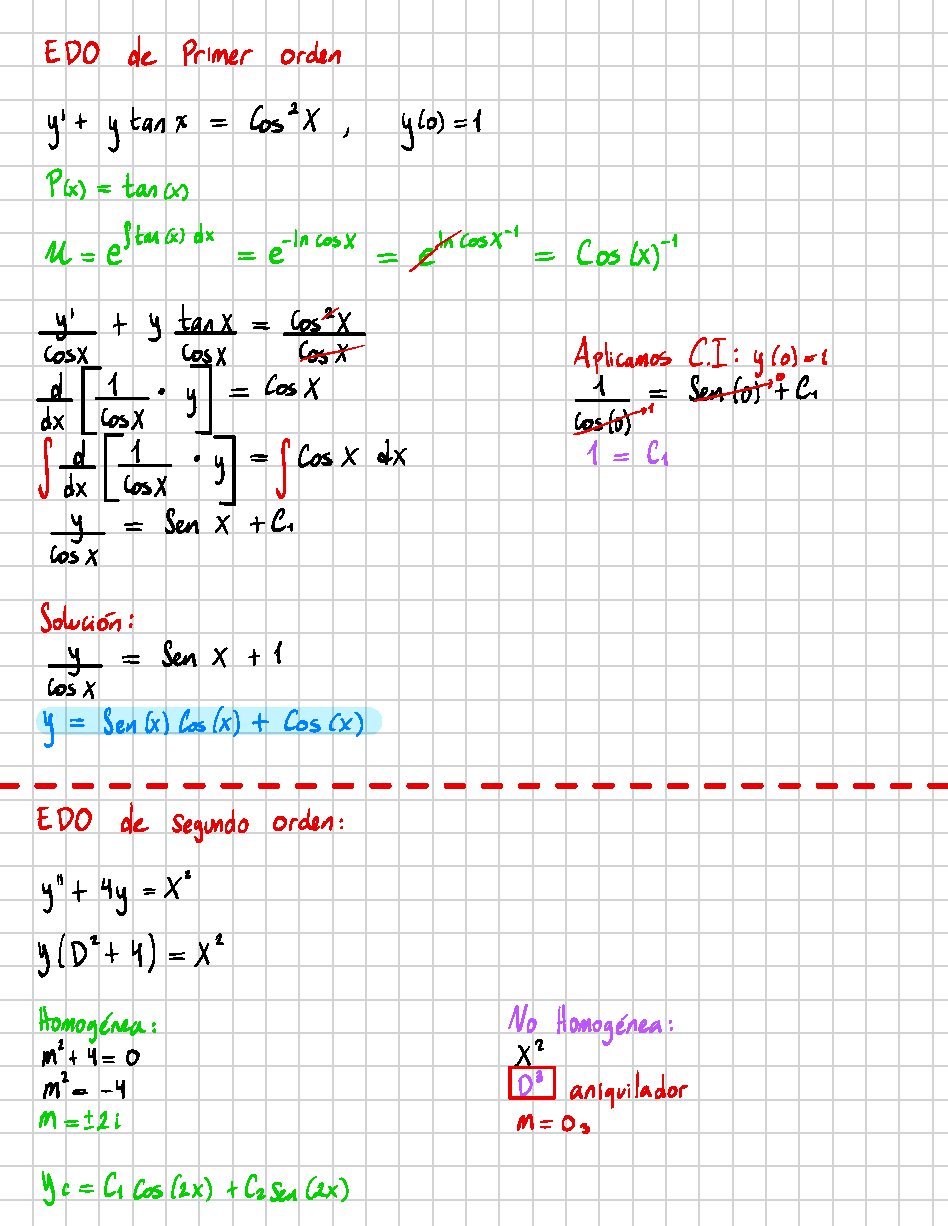
\includepdf[pages=-, scale=0.9, pagecommand={}]{recursos/Proyecto Final ED1 calculos.pdf}
	}{
		\textbf{Nota:} El archivo PDF de cálculos no se encontró en la ruta especificada.
	}
	
	\chapter{Bitácora de IA}
	Evidencia del uso de IA como copiloto en el desarrollo del proyecto.
	% Asegúrate de que este archivo exista en la carpeta recursos/
	\IfFileExists{recursos/Bitácora IA.pdf}{
		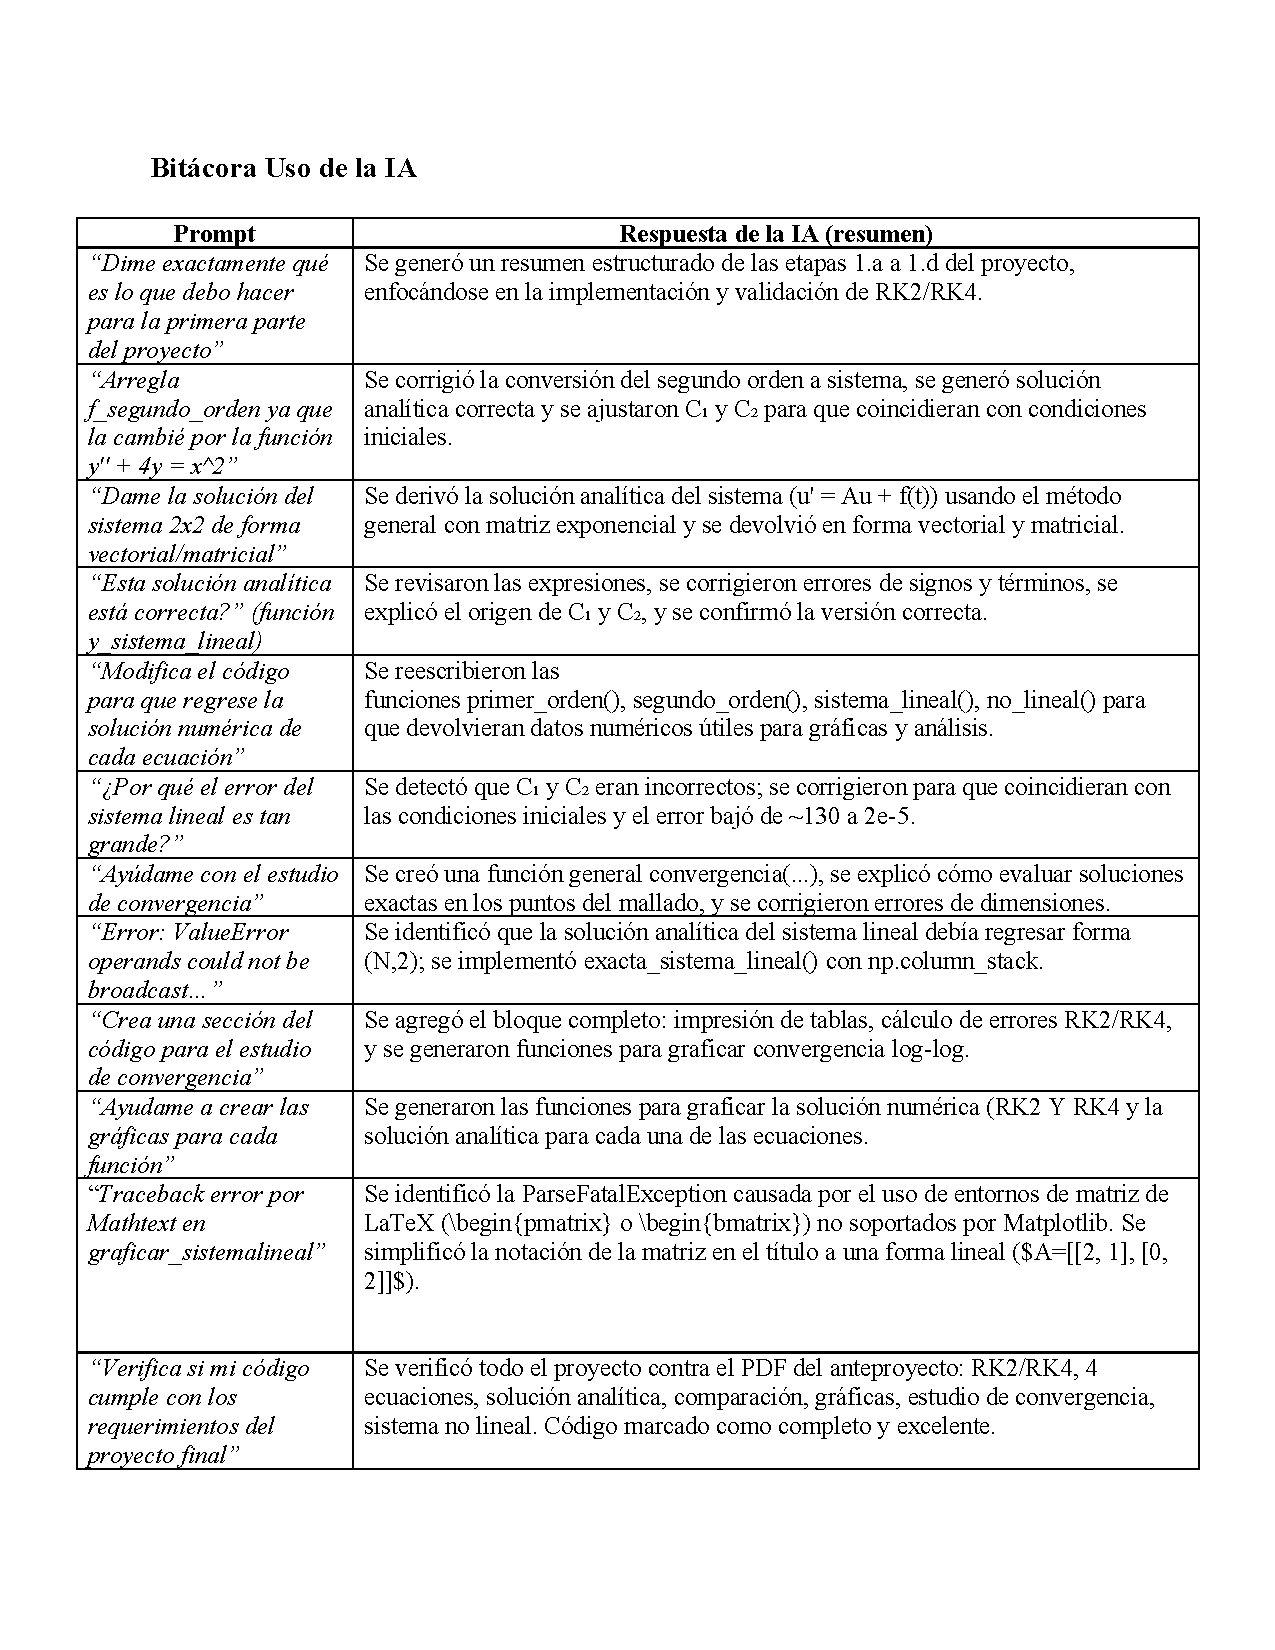
\includepdf[pages=-, scale=0.9, pagecommand={}]{recursos/Bitácora IA.pdf}
	}{
		\textbf{Nota:} El archivo PDF de bitácora no se encontró en la ruta especificada.
	}
	
	\chapter{Código Fuente (Python)}
	A continuación se presenta el código principal utilizado (`proyecto\_final.py`).
	
	\begin{lstlisting}[language=Python, caption=Implementación de Métodos Numéricos]
		import numpy as np
		import matplotlib.pyplot as plt
		
		# ==================
		# METODOS NUMERICOS
		# ==================
		def rk2_heun(f, t0, y0, h, n_steps):
		t = t0
		y = np.array(y0, dtype=float)
		ts = [t]
		ys = [y.copy()]
		for i in range(n_steps):
		k1 = f(t, y)
		y_euler = y + h * k1
		k2 = f(t + h, y_euler)
		y = y + (h/2.0)*(k1 + k2)
		t += h
		ts.append(t)
		ys.append(y.copy())
		return np.array(ts), np.array(ys)
		
		def rk4(f, t0, y0, h, n_steps):
		t = t0
		y = np.array(y0, dtype=float)
		ts = [t]
		ys = [y.copy()]
		for i in range(n_steps):
		k1 = f(t, y)
		k2 = f(t + h/2.0, y + h*k1/2.0)
		k3 = f(t + h/2.0, y + h*k2/2.0)
		k4 = f(t + h, y + h*k3)
		y = y + (h/6.0)*(k1 + 2*k2 + 2*k3 + k4)
		t += h
		ts.append(t)
		ys.append(y.copy())
		return np.array(ts), np.array(ys)
		
		# (El resto del codigo ha sido omitido por brevedad en el documento impreso, 
		# pero esta disponible completo en el repositorio GitHub).
	\end{lstlisting}
	
\end{document}